\documentclass[../main]{subfiles}

\begin{document}
\chapter{Prototype}
The prototype for this project is an end-to-end image classification pipeline for distinguishing two classes of mammographic scans using deep learning. Transfer learning is applied, with a pre-trained convolutional neural network being used for the classification of scans. The system ingests data from TFRecord files, originating from the DDSM dataset. These are then preprocessed for the model to use as input. The latter is then trained, and evaluated on this data.

\noindent The following is a summary of the prototype's data ingestion, and preprocessing pipelines.

\begin{itemize}
	\item \textbf{TFRecord Parsing} \textemdash\ A set of serialised examples from the DDSM dataset is parsed using TensorFlow's TFRecordDataset. Each example consists of three features: an image, a class label, and a normalised label.
	\item \textbf{Shuffling} \textemdash\ To improve stability in training, the dataset is shuffled with a buffer size of 31,000, and cached in memory for faster access across epochs.
	\item \textbf{Decoding, and Resizing} \textemdash\ Raw image bytes are kept in a unit8 tensor, and reshaped into a 299x299 image. OpenCV then resizes each image to 224x224 pixels, and replicates the single channel across three channels to form an RGB image, matching the requirements of the pre-trained model.
	\item \textbf{Dataset Conversion} \textemdash\ Images, and labels are converted into NumPy arrays X, and y for compatibility with Keras model training. Stratified splits are performed to split the dataset into training, validation, and test sets to maintain class balance. 
\end{itemize} 

\

\noindent The following details the CNN model's architecture, and definition.

\begin{itemize}
	\item \textbf{Basis} \textemdash\ The VGG16 architecture is used as a basis for the model, which is pretrained on ImageNet as the fixed feature extractor without the top classification layers. All convolutional layers of the VGG16 basis are non-trainable to retain the learned low-level, and mid-level features.
	\item \textbf{Custom Classifier Head} \textemdash\ On top of the frozen basis, a series of layers is added to form a custom classifier head. This consists of layers like dropout layers to manage overfitting, batch normalisation layers to improve training speed, and a dense layer with Glorot uniform initialisation, and a ReLU activation function for the final classification. The final output layer involves a sigmoid activation function for binary classification.
	\item \textbf{Compilation} \textemdash\ The final model is compiled with the Adam optimiser, binary cross-entropy loss, and accuracy as the prime metric.
\end{itemize}

\begin{lstlisting}[language=Python, caption={Prototype model definition.}]
base_model = VGG16(
	weights="imagenet", include_top=False, input_shape=(IMAGE_SIZE, IMAGE_SIZE, 3)
)  # Base model VGG16 pretrained on ImageNet
base_model.trainable = False

""" Custom classification head """
model = Sequential(
	[
	    base_model,
	    Dropout(0.5),  # Dropout layers to prevent overfitting
	    Flatten(),
	    BatchNormalization(),  # Stabilises learning
	    Dense(
		1024, kernel_initializer=GlorotUniform()
	    ),  # Learn decision boundaries
	    BatchNormalization(),
	    Activation("relu"),
	    Dropout(0.5),
	    Dense(512, kernel_initializer=GlorotUniform()),
	    BatchNormalization(),
	    Activation("relu"),
	    Dropout(0.5),
	    Dense(1, activation="sigmoid"),  # Output layer for binary classification
	]
)

model.compile(
	optimizer="adam", loss="binary_crossentropy", metrics=["accuracy"]
)  # Compile the model with Adam optimizer, binary crossentropy loss, and accuracy metric
\end{lstlisting}

\noindent Note that this prototype borrows inspiration from the following work \\ \textit{https://www.youtube.com/watch?v=mmGy\_tZU3lc}.

\section{Evaluation}
The system was evaluated using a primarily quantitative performance metrices.

\begin{itemize}
	\item \textbf{Accuracy} \textemdash\ The prototype achieved an accuracy of 0.89 in testing on a held-out test set.
	\item \textbf{Precision, Recall, and F1-score} \textemdash\ Using macro-averaging across the two classes, precision, recall, and F1-score were used to account for any class imbalance.
	\item \textbf{ROC AUC} \textemdash\ The receiver operating characteristic (ROC) curve, and the macro-averaged area under the curve (AUC) were determined to assess the model's discrimination threshold independently of any single decision threshold.
\end{itemize}

\noindent In terms of ROC analysis, the model achieved an AUC value of 0.89, demonstrating a solid separability between the two classes at various thresholds.

\section{Discussion of Results}
In general, the prototype demonstrates feasibility of the proposed classification approach. The frozen backbone makes it easier to train the model, and lessens computational cost, but limits the model's ability to adapt to domain-specific features. In addition, the custom classifier head learns to distinguish classes understandably well.

\begin{figure}[h]
	\centering
	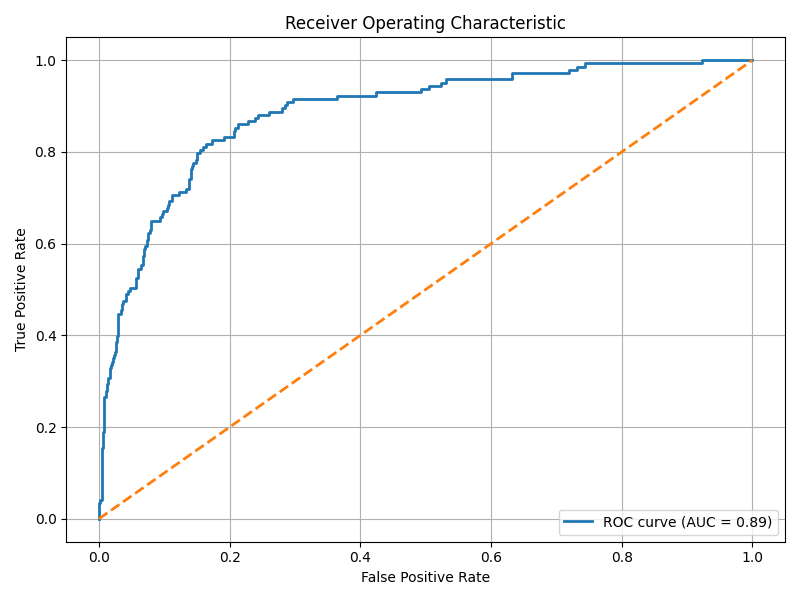
\includegraphics[width=0.8\textwidth]{assets/roc.png}
	\caption{Diagram of the ROC curve for the prototype model.}
	\label{fig:prototype_architecture}
\end{figure}

\begin{itemize}
	\item Rapid prototyping using transfer learning enabled end-to-end functionality rapidly.
	\item Quantitative metrics like accuracy, precision, recall, F1-score, and AUC indicate sufficient performance for the initial project.
\end{itemize}

\begin{table}[h]
	\centering
	\begin{tabular}{|c|c|c|c|c|}
		\hline
		Metric & Value \\
		\hline
		Accuracy & 0.89 \\
		Precision & 0.55 \\
		Recall & 0.61 \\
		F1-score & 0.58 \\
		AUC & 0.89 \\
		\hline
	\end{tabular}
	\caption{Quantitative performance metrics of the prototype model.}
	\label{tab:prototype_metrics}
\end{table}

\noindent Note that these results were achieved with the limited training parameters of 1 epoch, and a batch size of 10. The performance of this model is expected to improve with further training, and optimisation.

\section{Future Work}
This prototype serves as a basic proof-of-concept, and a foundation for future work. The final system will require further refinement, and optimisation, as well as additional features, and functionality to make it more user-friendly, and robust.

\begin{itemize}
	\item \textbf{Model Optimisation} \textemdash\ The model can be further optimised by adjusting its architecture, and increasing the number of epochs.
	\item \textbf{Advanced Architectures} \textemdash\ Alternative architectures could be experimented with like ResNet50, and EfficientNet that may offer better performance.
	\item \textbf{Data Augmentation} \textemdash\ tf.image operations like random flips, rotations, and brightness adjustments could be introduced to improve generalisation.
	\item \textbf{User Interface} \textemdash\ A user-friendly interface can be developed to allow users to easily upload images, and view results.
	\item \textbf{Deployment} \textemdash\ The model can be deployed as a web service through REST APIs, and be inferenced through them for user-friendly accessibility, particularly for clinical settings.
	\item \textbf{CI/CD} \textemdash\ Implementing continuous integration, and continuous deployment (CI/CD) practices such as the introduction of containerisation with Docker will ensure that the system is easily maintainable, scalable, and transferable across different platforms.
\end{itemize}

\newpage

\section{Approximate Plan of Work}
The following is an approximate plan of work for the next stages of the project. It is subject to change, depending on the progress, and exigencies of it.

\newcolumntype{L}[1]{>{\raggedright\arraybackslash}p{#1}}

\begin{table}[ht]
\centering
\begin{adjustbox}{width=\textwidth}
\begin{tabularx}{\textwidth}{|L{3.2cm}|X|X|L{1.8cm}|L{1.8cm}|L{1.8cm}|}
\hline
\textbf{Task} & \textbf{Description} & \textbf{Approx. Duration} & \textbf{Start Date} & \textbf{End Date} \\
\hline
Model Optimisation & Tune hyperparameters, increase epochs, and batch size & 2 weeks & Jun 16, 2025 & Jun 27, 2025 \\
\hline
Advanced Architectures & Experiment with ResNet50, EfficientNet, or ViTs & 3 weeks & Jun 30, 2025 & Jul 18, 2025 \\
\hline
	User Interface Development & Build web UI for image uploads, and results together with endpoints & 2 weeks & Jul 21, 2025 & Aug 1, 2025\\
\hline
Deployment via REST API & Finalise Django REST API backend & 2 weeks &  Aug 4, 2025 & Aug 18, 2025\\
\hline
CI/CD Integration & Containerise with Docker & 2 weeks &  Aug 19, 2025 & Aug 22, 2025\\
\hline
\end{tabularx}
\end{adjustbox}
\caption{Approximate Planned Timeline for the Project}
\label{tab:project_timeline}
\end{table}


\end{document}
